\appendix
\section{Sensitivity, robustness and reproduction}
\label{sec:appendix}

Several sweeps and specification variants are reported here, each re-running the full pipeline on the realised 2026 central scenario against the same baseline. They are presented in order of how much they move the answer, and that ordering is the appendix's main message. It has been inverted by this revision, and the inversion matters enough to state at the top.

Earlier versions of this appendix instructed the reader to direct scepticism at the demand-elasticity assumption and nowhere else. That instruction was an artefact of measuring demand response as a change in \emph{expenditure} rather than as a change in \emph{welfare}: a household that stops heating its home spends less, and counting that as a saving is exactly the ``heat or eat'' fallacy this appendix criticises elsewhere. Measured as a money-metric welfare loss --- bounded above by the Laspeyres term and below by the Paasche term --- demand response removes at most \genWelfareShavedHighEpsPct{} per cent of the loss at the most elastic point of the grid, not the \genSpendShavedHighEpsPct{} per cent the expenditure measure suggested.

\textbf{The honest uncertainty ranking is therefore: the motor-fuel and domestic-energy imputations first, the accounting basis --- phase-in against steady state, equivalised against unequivalised --- second, the pass-through and damping calibration third, and the demand elasticity a distant fourth.} A reader deciding where to direct scepticism should direct it at the first three.

No constituency-level robustness statistic appears in this appendix. The data release carries no constituency weight matrix, so seat-level rank correlations are not computable and none has been substituted (Section~\ref{sec:step3}).

\subsection{Demand response: smaller than it looked}
\label{app:elasticity}

The main specification is zero-elasticity by construction: equation~\eqref{eq:firstorder} evaluates the price change at pre-shock quantities, which is the \citet{deaton1980} first-order approximation and an explicit upper bound on the welfare loss. Elasticity is therefore a robustness check on the main result, not an alternative main result --- an important framing point, because an elasticity-adjusted central estimate would be a number driven by a parameter this paper does not estimate.

The sweep applies the constant-elasticity spend factor $(p_1/p_0)^{1+\varepsilon}$ --- never a linear approximation, which would misbehave at the top of the grid --- over a flat grid from $\varepsilon = 0$ to $\varepsilon = -0.8$, and additionally under five named published specifications: Labandeira, Labeaga and L\'opez-Otero's short- and long-run per-carrier means, Priesmann and Praktiknjo's income-varying short and long run, and a decile-varying configuration replicating an earlier published application of the same elasticities.

\paragraph{Magnitude, measured correctly.} The quantity that matters is the compensating variation, not the change in spending. The two differ by exactly the amount a household saves by consuming less, which is a welfare loss to that household rather than a costless adjustment, and the gap between them is what made this sweep look dominant. Bounding the compensating variation between the Laspeyres term evaluated at pre-shock quantities and the Paasche term evaluated at post-shock quantities, the aggregate welfare loss runs from \pounds\genElasticityAggZeroBn{} billion at $\varepsilon = 0$ to \pounds\genCvLowerHighEpsBn{} billion at $\varepsilon = -0.8$ --- a reduction of \genWelfareShavedHighEpsPct{} per cent at the extreme end of a grid whose extreme end is not a credible short-run value in any case. On the expenditure measure the same endpoint removed \genSpendShavedHighEpsPct{} per cent of the loss. That figure has been withdrawn; it counted foregone heating as costless.

\paragraph{The credible short-run band is narrower still.} The published short-run estimates cluster tightly, and on the welfare measure they barely move the headline: Labandeira's short-run per-carrier means shave \genLabandeiraShortWelfareShaved{} per cent off the zero-elasticity figure and Priesmann's income-varying short run \genPriesmannShortWelfareShaved{} per cent. Both sweeps run on the main specification, so the grid is anchored at its \pounds\genElasticityAggZeroBn{} billion zero-elasticity figure. A reader who rejects the zero-elasticity headline outright therefore lands close to it rather than somewhere qualitatively different. Labandeira's \emph{long}-run figures shave more, but they embed appliance and vehicle stock turnover and are the wrong horizon for a 2026 spike; they bound the exercise and are not a candidate headline.

\paragraph{What does not change.} Nothing about the distributional story. A flat elasticity rescales every decile by the same factor, so the decile-one to decile-ten percentage ratio is unchanged across the entire flat grid. The income-varying specifications \emph{do} flatten the gradient --- Priesmann's takes the ratio from \genDecileRatioPct{} to \genPriesmannDecileRatio{} to one --- because poor households are modelled as the ones with room to cut back. That flattening is precisely the ``heat or eat'' objection in numerical form: it treats involuntary rationing as welfare-neutral substitution, and treating a household that cannot afford to heat its home as having merely revealed a preference is the substantive reason this paper keeps the upper bound as its headline. Either way the qualitative ordering survives every row of the sweep: the poor lose more in percentage terms and less in cash in all fourteen specifications.

\begin{figure}[htbp]
\centering
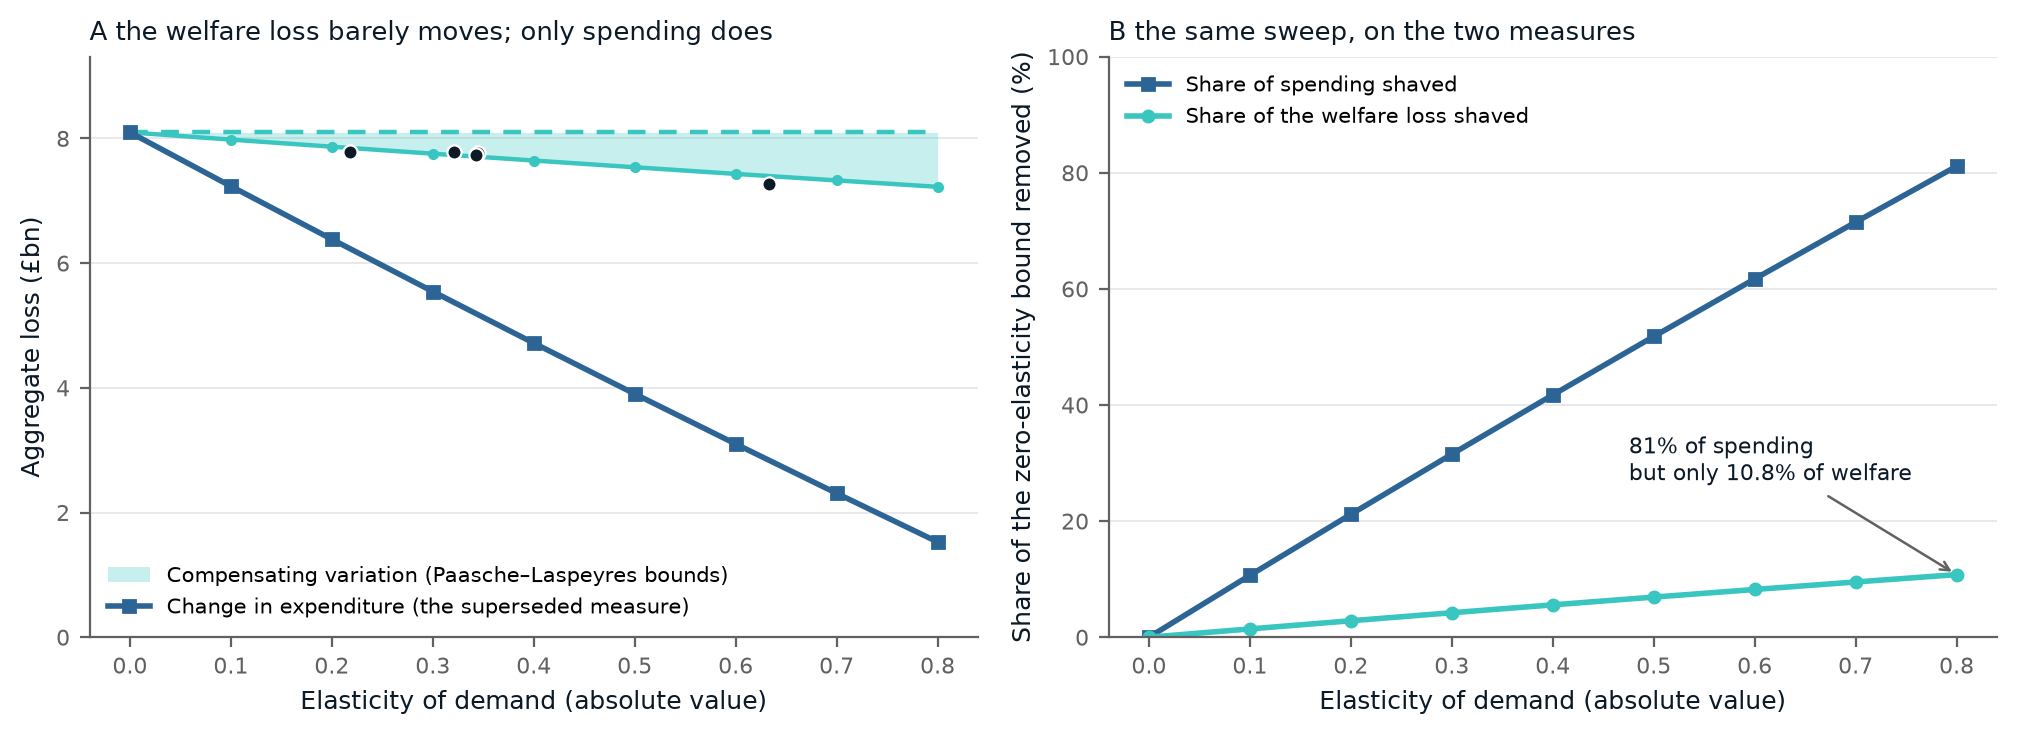
\includegraphics[width=\textwidth]{../results/figures/figA2_welfare_bounds.png}
\caption{Why the demand-response sweep is not the paper's largest uncertainty. Panel A places the change in expenditure --- the measure an earlier draft reported as the loss --- inside the Paasche--Laspeyres bounds on the compensating variation. Panel B shows the two on the same scale: at the strongest response in the grid, four fifths of the \emph{spending} disappears and about a tenth of the \emph{welfare loss} does. The difference is foregone consumption the household valued.}
\label{fig:welfarebounds}
\end{figure}

% tab_elasticity.tex — machine-generated by analysis/emit_tables.py
% generated 2026-08-26T12:16:39Z from results/ (central scenario: realised_2026). DO NOT EDIT BY HAND.
% A complete table float, caption and label included: the appendix inputs this directly. Requires \usepackage{booktabs}.
\begin{table}[htbp]
\centering
\caption{Demand-response sweep, realised 2026 scenario. The main specification is zero elasticity, an explicit upper bound on the welfare loss; every other row is a robustness check, not an alternative headline. The level of the loss moves by a factor of five across the grid; the qualitative decile ordering does not move at all.}
\label{tab:elasticity}
\begin{tabular}{lrrrrrr}
\toprule
Specification & Mean $\varepsilon$ & Mean loss (\pounds) & \% of income & Aggregate (\pounds bn) & Decile 1 (\%) & Decile 10 (\%) \\
\midrule
Labandeira et al., short run & $-$0.22 & 344 & 0.57 & 10.15 & 1.51 & 0.26 \\
Labandeira et al., long run & $-$0.63 & 134 & 0.22 & 3.94 & 0.58 & 0.10 \\
Priesmann and Praktiknjo, short run & $-$0.32 & 320 & 0.53 & 9.42 & 1.05 & 0.29 \\
Priesmann and Praktiknjo, long run & $-$0.34 & 314 & 0.52 & 9.25 & 1.08 & 0.28 \\
Prior-repository replication & $-$0.34 & 304 & 0.50 & 8.95 & 0.70 & 0.32 \\
Flat $\varepsilon = 0$ (main specification) & 0.00 & 471 & 0.77 & 13.89 & 2.07 & 0.36 \\
Flat $\varepsilon = -0.1$ & $-$0.10 & 420 & 0.69 & 12.36 & 1.84 & 0.32 \\
Flat $\varepsilon = -0.2$ & $-$0.20 & 369 & 0.61 & 10.87 & 1.62 & 0.28 \\
Flat $\varepsilon = -0.3$ & $-$0.30 & 319 & 0.53 & 9.42 & 1.40 & 0.24 \\
Flat $\varepsilon = -0.4$ & $-$0.40 & 271 & 0.45 & 7.99 & 1.19 & 0.21 \\
Flat $\varepsilon = -0.5$ & $-$0.50 & 223 & 0.37 & 6.59 & 0.98 & 0.17 \\
Flat $\varepsilon = -0.6$ & $-$0.60 & 177 & 0.29 & 5.21 & 0.78 & 0.14 \\
Flat $\varepsilon = -0.7$ & $-$0.70 & 131 & 0.22 & 3.87 & 0.58 & 0.10 \\
Flat $\varepsilon = -0.8$ & $-$0.80 & 87 & 0.14 & 2.55 & 0.38 & 0.07 \\
\bottomrule
\end{tabular}
\end{table}


\begin{figure}[htbp]
\centering
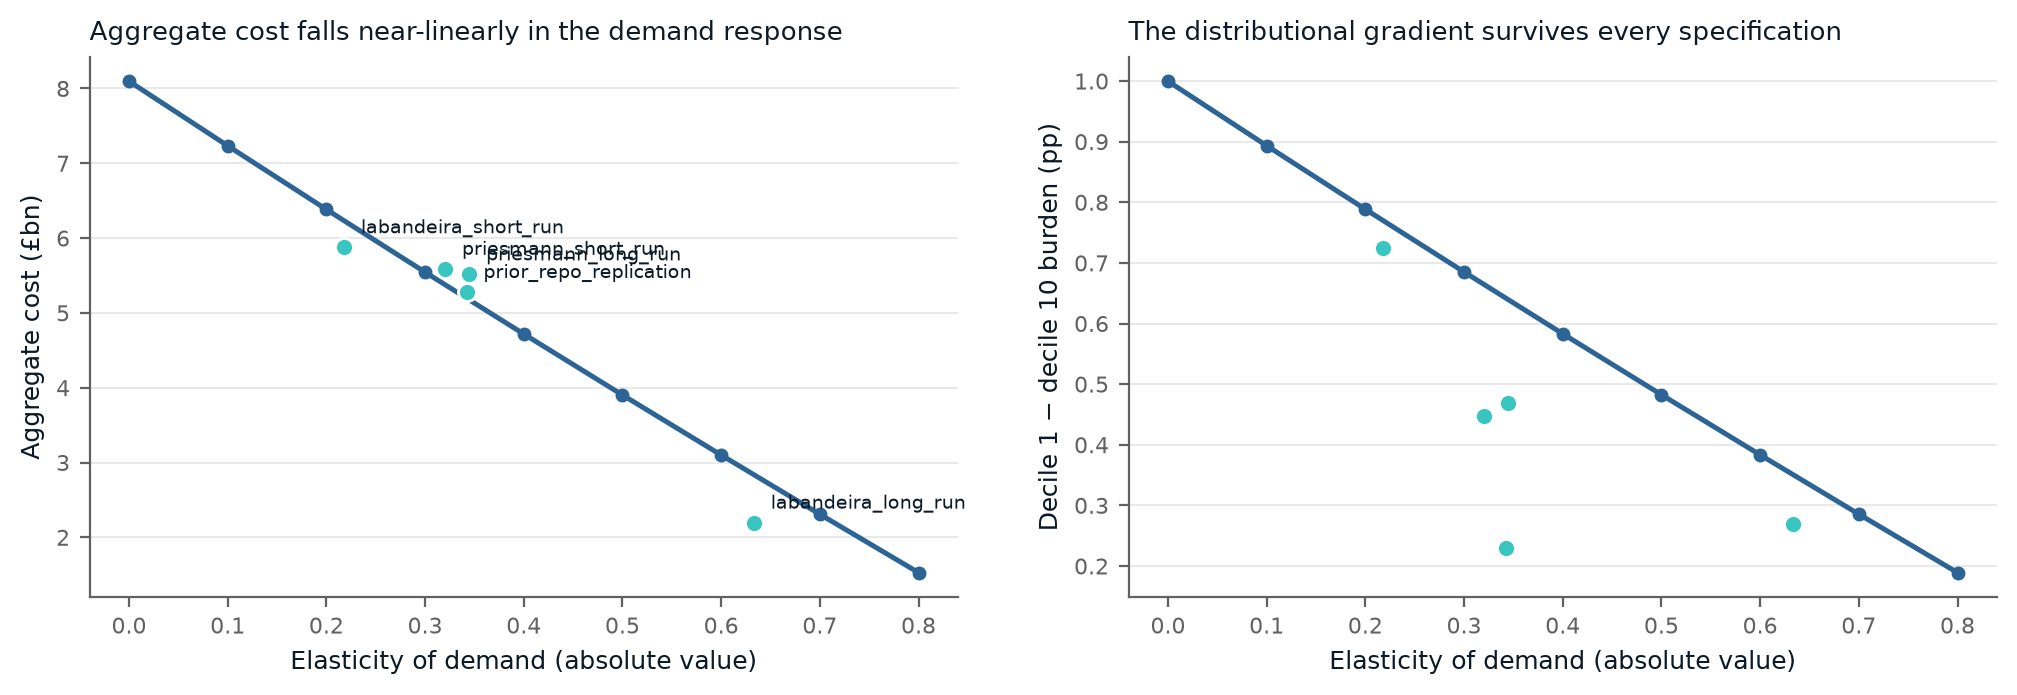
\includegraphics[width=.85\textwidth]{../results/figures/figA1_elasticity.png}
\caption{Decile incidence profile under each elasticity specification. The parallel spacing of the flat-grid lines shows that the distributional conclusions are invariant to a uniform elasticity assumption even where the level of the loss is not; the income-varying specifications flatten the gradient, for the reason discussed in the text.}
\label{fig:elasticity}
\end{figure}

A caveat on the exercise itself: applying a constant elasticity to a capped price is not innocuous, because households facing a standing charge plus a unit rate face a marginal price that differs from their average price, and the block designs scored in Section~\ref{sec:policy} change the marginal price for some households and not others. The sweep is fed the same bill factor as the main specification, not a unit rate --- an earlier version of this appendix claimed the latter --- and it does not model standing-charge effects, which would make the marginal price move by more than the bill does.

\subsection{Specification variants of the central scenario}
\label{app:specvariants}

Seven calibrations of the realised 2026 scenario are carried through the paper rather than one, and this subsection states what separates them so that any figure quoted in the text can be located. Table~\ref{tab:specifications} reports them on a common set of statistics. All seven are annualised over the same window, March 2026 to February 2027; none is a calendar-year figure.

The single statistic the seven are carried for is the motor-fuel share of the aggregate loss, and the range is the result rather than any point in it. Setting the peak-fuel upper bound aside --- it is a bound, not a candidate headline --- the share runs from \genSymDampMotorFuelShareOfLoss{} per cent under symmetric damping to \genMotorFuelShareOfLoss{} per cent in the main specification, with the ONS-levels calibration at \genOnsLevelsMotorFuelShareOfLoss{} per cent in between; including the peak-fuel row takes the top of the range to \genSpecFuelShareMaxPct{} per cent. The paper quotes the range. Motor fuel carries a large share on every calibration and a majority on most of them, and \genMotorFuelShareOfLoss{} per cent is not offered as settled.

\begin{table}[htbp]
\centering
\caption{The seven calibrations of the realised 2026 scenario, on a common set of statistics. The main specification applies the equivalised after-housing-costs denominator and the consumption-weighted quarterly cap average; each of the others varies one accounting or imputation choice from it.}
\label{tab:specifications}
% tab_specifications.tex — machine-generated by analysis/emit_tables.py
% generated 2026-08-27T09:07:01Z from results/ (central scenario: realised_2026). DO NOT EDIT BY HAND.
% A standalone tabular: \input this inside a table float that carries the caption and label. Requires \usepackage{booktabs}.
{\small\setlength{\tabcolsep}{2.6pt}
\begin{tabular}{lrrrrrrrrr}
\toprule
Specification & \begin{tabular}[b]{@{}c@{}}Agg. \\ (\pounds bn)\end{tabular} & \begin{tabular}[b]{@{}c@{}}Mean \\ (\pounds)\end{tabular} & \begin{tabular}[b]{@{}c@{}}Mean \\ (\%)\end{tabular} & \begin{tabular}[b]{@{}c@{}}D1 \\ (\pounds)\end{tabular} & \begin{tabular}[b]{@{}c@{}}D1 \\ (\%)\end{tabular} & \begin{tabular}[b]{@{}c@{}}D10 \\ (\pounds)\end{tabular} & \begin{tabular}[b]{@{}c@{}}D10 \\ (\%)\end{tabular} & \begin{tabular}[b]{@{}c@{}}D1/D10 \\ (\%)\end{tabular} & \begin{tabular}[b]{@{}c@{}}Motor fuel \\ (\% of loss)\end{tabular} \\
\midrule
Main specification & 8.10 & 275 & 0.60 & 231 & 2.29 & 314 & 0.25 & 9.22 & 75.6 \\
Steady state & 8.59 & 292 & 0.64 & 245 & 2.44 & 333 & 0.26 & 9.22 & 71.3 \\
Symmetric damping & 12.57 & 427 & 0.94 & 354 & 3.59 & 490 & 0.39 & 9.25 & 48.7 \\
Peak fuel (upper bound) & 11.39 & 387 & 0.85 & 326 & 3.22 & 441 & 0.35 & 9.21 & 82.7 \\
ONS shape & 8.13 & 276 & 0.61 & 140 & 1.41 & 473 & 0.37 & 3.75 & 75.7 \\
ONS both levels & 7.52 & 255 & 0.56 & 140 & 1.43 & 417 & 0.33 & 4.32 & 64.9 \\
Unequivalised & 8.10 & 275 & 0.45 & 231 & 1.16 & 314 & 0.21 & 5.53 & 75.6 \\
\bottomrule
\end{tabular}
}

\end{table}


The \emph{main} specification takes the annual domestic price as the consumption-weighted average of the quarterly cap levels prevailing over the modelled window of March 2026 to February 2027, damps both the wholesale gas peak and the observed pump-price peak to annual averages at sustained fractions of \genGasSustainedFraction{} and \genPumpSustainedFraction{} per cent respectively, and divides every percentage by equivalised net income after housing costs. It gives an aggregate loss of \pounds \genAggSpendRealisedBn{} billion, a mean household loss of \pounds \genCentralLossMean{} (\genCentralLossPctIncome{} per cent of income), a motor-fuel share of \genMotorFuelShareOfLoss{} per cent, and a decile-one to decile-ten burden ratio of \genDecileRatioPct{} to one.

The \emph{steady-state} specification charges the level the cap eventually reaches for the whole of the modelled window rather than the phased-in average --- which is what the code did before this revision, in contradiction of the method the paper describes. It gives \pounds \genSteadyStateAggBn{} billion, \pounds \genSteadyStateLossMean{} (\genSteadyStateLossPctIncome{} per cent), a motor-fuel share of \genSteadyStateMotorFuelShareOfLoss{} per cent and a ratio of \genSteadyStateDecileRatioPct{} to one. It is reported because it is the specification the earlier draft's headline figures came from, and because it is a defensible answer to a different question --- what an indefinitely sustained shock would cost --- rather than to the twelve-months-from-the-shock question this paper asks.

The \emph{symmetric-damping} specification is the one that most threatens the paper's compositional claim, and it is reported for that reason. It damps the gas and pump peaks by a \emph{common} fraction rather than by the fuel-specific pair the main specification uses, which is what a reader unpersuaded by the argument in Section~\ref{sec:step1} would impose. It gives \pounds \genSymDampAggBn{} billion, \pounds \genSymDampLossMean{} (\genSymDampLossPctIncome{} per cent), a ratio of \genSymDampDecileRatioPct{} to one --- and a motor-fuel share of \genSymDampMotorFuelShareOfLoss{} per cent, which is a minority. Combined with the steady-state basis it gives \genSymDampSteadyMotorFuelShare{} per cent and combined with ONS-consistent spending levels \genSymDampOnsLevelsMotorFuelShare{} per cent. The motor-fuel share depends on the \emph{ratio} of the two damping fractions and on little else, so this single choice moves the composition result more than any other in the paper while leaving the distributional result untouched.

The \emph{peak-fuel} specification is the upper bound: it applies the observed peak pump prices undamped for a full year, giving \pounds \genPeakFuelAggBn{} billion, \pounds \genPeakFuelLossMean{} (\genPeakFuelLossPctIncome{} per cent), a motor-fuel share of \genPeakFuelMotorFuelShareOfLoss{} per cent, and a ratio of \genPeakFuelDecileRatioPct{} to one. It is not a candidate headline: charging households an annual average pump price equal to a peak that lasted part of the year is a larger shock than the one that occurred, not a bound on it.

\begin{table}[htbp]
\centering
\caption{The calibrations of the realised 2026 scenario compared: the main specification, the steady-state accounting basis, symmetric damping, the peak-fuel upper bound, the two ONS calibrations, and the unequivalised robustness line.}
\label{tab:variants}
% tab_variants.tex — machine-generated by analysis/emit_tables.py
% generated 2026-08-27T12:30:25Z from results/ (central scenario: realised_2026). DO NOT EDIT BY HAND.
% A standalone tabular: \input this inside a table float that carries the caption and label. Requires \usepackage{booktabs}.
{\small\setlength{\tabcolsep}{4.5pt}
\begin{tabular}{lrrrr}
\toprule
 & \begin{tabular}[b]{@{}c@{}}Main \\ specification\end{tabular} & \begin{tabular}[b]{@{}c@{}}Peak-fuel \\ upper bound\end{tabular} & \begin{tabular}[b]{@{}c@{}}ONS-calibrated \\ motor fuel\end{tabular} & \begin{tabular}[b]{@{}c@{}}Calendar 2026 \\ (RF window)\end{tabular} \\
\midrule
Aggregate additional spend (\pounds bn) & 11.10 & 14.39 & 11.13 & 9.13 \\
Mean loss (\pounds) & 377 & 488 & 378 & 310 \\
Mean loss (\% of income) & 0.83 & 1.07 & 0.83 & 0.68 \\
\midrule
Decile 1 loss (\pounds) & 313 & 409 & 222 & 259 \\
Decile 1 loss (\% of income) & 3.16 & 4.09 & 2.27 & 2.60 \\
Decile 10 loss (\pounds) & 432 & 559 & 591 & 355 \\
Decile 10 loss (\% of income) & 0.34 & 0.44 & 0.47 & 0.28 \\
Decile 1/10 ratio (\% of income) & 9.24 & 9.23 & 4.86 & 9.23 \\
\quad from decile 2 (D2/D10) & 4.46 & 4.31 & 3.01 & 4.37 \\
\quad D1/D10, winsorised & 11.42 & 11.49 & 5.92 & 11.46 \\
\quad D2/D10, winsorised & 4.51 & 4.35 & 3.04 & 4.42 \\
\midrule
Gas share of loss (\%) & 24.8 & 19.1 & 24.7 & 20.9 \\
Electricity share of loss (\%) & 20.1 & 15.5 & 20.0 & 18.0 \\
Motor fuel share of loss (\%) & 55.2 & 65.4 & 55.3 & 61.0 \\
\midrule
Means-tested share of loss (\%) & 5.22 & 4.59 & 4.91 & 4.85 \\
\bottomrule
\end{tabular}
}

\end{table}

The two \emph{ONS} specifications address the imputation defects of Section~\ref{sec:limitations}. The first rescales the decile \emph{shape} of motor-fuel spending to the ONS Family Spending FYE 2025 profile. The rescaling preserves the microdata's national total and transplants only the ONS shape, so the rescaled decile levels --- \pounds \genRescaledFuelDecileOneGbp{} at the bottom against \pounds \genRescaledFuelDecileTenGbp{} at the top --- sit well above the ONS levels whose shape they borrow (\pounds \genOnsBenchFuelDecileOneGbp{} and \pounds \genOnsBenchFuelDecileTenGbp{}); an earlier draft quoted the rescaled figures three times as though they were the ONS benchmark, and they are not. Correcting the shape alone: it barely moves the aggregate, at \pounds \genOnsFuelAggBn{} billion and \pounds \genOnsFuelLossMean{} (\genOnsFuelLossPctIncome{} per cent) with a motor-fuel share of \genOnsFuelMotorFuelShareOfLoss{} per cent, and moves the distribution a great deal: decile one falls from \genDecileOneLossPct{} to \genOnsFuelDecileOneLossPct{} per cent of income, decile ten \emph{rises} from \genDecileTenLossPct{} to \genOnsFuelDecileTenLossPct{} per cent (in cash, from \pounds \genDecileTenLossGbp{} to \pounds \genOnsFuelDecileTenLossGbp{}), and the ratio falls to \genOnsFuelDecileRatioPct{} to one. The second corrects both spending \emph{levels} as well --- motor fuel down, domestic energy up --- giving \pounds \genOnsLevelsAggBn{} billion, \pounds \genOnsLevelsLossMean{} (\genOnsLevelsLossPctIncome{} per cent), a motor-fuel share of \genOnsLevelsMotorFuelShareOfLoss{} per cent and a ratio of \genOnsLevelsDecileRatioPct{} to one. Together they are the relevant robustness tests for every distributional magnitude in the paper, and the reason those magnitudes are reported as uncertain by roughly a factor of two.

The \emph{unequivalised} line is not an alternative specification but a visibility device. Dividing by raw household net income rather than by equivalised net income after housing costs --- which is what the code did before this revision, while the text claimed otherwise --- gives a mean burden of \genUnequivLossPctIncome{} per cent, a decile-one burden of \genUnequivDecileOneLossPct{} per cent against \genUnequivDecileTenLossPct{} per cent in decile ten, and a ratio of \genUnequivDecileRatioPct{} to one against \genDecileRatioPct{} on the equivalised basis. It is reported once so that the effect of the correction can be seen rather than inferred.

\subsection{Cap lag: a real sensitivity, now small}
\label{app:caplag}

The lag $\ell$ in equation~\eqref{eq:passthrough} places the quarterly phase-in profile on the calendar. It is the paper's most contestable calibration, so it is swept over one to four quarters against the loss annualised on the paper's own window --- March 2026 to February 2027 --- and the sweep is the paper's reconciliation as well as its sensitivity check. The domestic-energy channel is lagged; motor fuel is not, because pump prices pass through in weeks.

Two things about this subsection have changed, and the first is structural. The phase-in profile is now computed \emph{from} $\ell$ rather than written down as a fixed tuple alongside it. Previously the two were disconnected: the cumulative weight applied to the profile carried no lag dependence at all, so the invariance this appendix reported was an identity of the construction rather than a finding about the world, and the same disconnection was what allowed the headline and this sweep to disagree by roughly half. The profile now follows the lag, the sweep asserts that its central row reproduces the headline exactly, and the invariance it reports is therefore a measured residual rather than a guaranteed zero.

\paragraph{What the sweep now finds.} The mean household loss runs from \pounds\genCapLagAnnualisedLagOne{} at $\ell = 1$ to \pounds\genCapLagAnnualisedLagFour{} at $\ell = 4$, with the paper's $\ell = 1.5$ giving \pounds\genCapLagAnnualisedPaper{} --- which is the headline figure of \pounds \genCentralLossMean{}, by assertion rather than by coincidence. The spread across the whole range is \pounds \genCapLagRangeGbp{} per household, \genCapLagSpreadPct{} per cent of the central figure. That is a real sensitivity and a small one, and the reason it is small is the window: with both legs annualised over the twelve months from the shock, a shift in where the cap profile starts moves how much of the domestic pass-through falls inside a window that contains both cap resets either way. Under the earlier mismatched windows the same shift moved the answer by roughly fifty per cent, because a calendar-2026 window clipped the domestic leg exactly where the lag placed it.

\paragraph{Anchored against unanchored.} The sweep is run twice, and the pair is what shows how much of the small spread is the anchor doing its work. In the \emph{anchored} rows the gas sustained fraction is re-solved at each lag so that the modelled October cap continues to reproduce Ofgem's confirmed level \citep{ofgem2026cap} --- which is what the main specification does, since the fraction is solved rather than assumed (Section~\ref{sec:step1}). In the \emph{unanchored} rows the fraction is held at its central value while the lag moves, so the modelled cap drifts away from the confirmed one. The anchored spread is \pounds \genCapLagRangeGbp{} (\genCapLagSpreadPct{} per cent); the unanchored spread is \pounds \genCapLagRangeUnanchoredGbp{} (\genCapLagSpreadUnanchoredPct{} per cent), roughly twice as wide, and it widens monotonically with the lag because a longer lag pushes more of the profile past the anchor quarter and the fraction is no longer free to compensate. The anchor is therefore not cosmetic: it absorbs about half the lag sensitivity by construction, and it does so by holding the one quantity in the domestic leg that is externally observed.

Two consequences for how the paper's numbers should be read. First, any annual figure in this paper is lag-sensitive by \genCapLagSpreadPct{} per cent, which is smaller than the specification spread of Appendix~\ref{app:specvariants} and much smaller than the imputation uncertainty, so the lag has moved from the top of the uncertainty ranking to near the bottom. Second, the composition still moves more than the level does: the motor-fuel share of the loss runs across the swept range in the same direction, because a longer lag defers domestic pass-through while the pump leg does not move, which is the same calibration dependence Section~\ref{sec:results-fuel} reports arriving here from a third direction.

% tab_caplag.tex — machine-generated by analysis/emit_tables.py
% generated 2026-08-27T09:07:01Z from results/ (central scenario: realised_2026). DO NOT EDIT BY HAND.
% A complete table float, caption and label included: the appendix inputs this directly. Requires \usepackage{booktabs}.
\begin{table}[htbp]
\centering
\caption{Wholesale-to-retail lag sweep, realised 2026 scenario, on both anchoring rules. ``Anchored'' re-solves the sustained fraction at each lag so the Cornwall cap anchor still binds; ``unanchored'' holds it at the central value and so varies the timing alone. The cumulative burden is invariant along the unanchored series --- an identity, since the phase-in weights only move the burden between calendar years --- so what moves in the columns below is the attribution to the modelled year, not the size of the shock. The two rules agree to two quarters and separate after, which is where the anchoring rule rather than the lag is doing the work.}
\label{tab:caplag}
{\small\setlength{\tabcolsep}{4.5pt}
\begin{tabular}{llrrrrr}
\toprule
& & \multicolumn{2}{c}{Booked in the modelled year} & \multicolumn{2}{c}{By leg (\pounds bn)} & \\
\cmidrule(lr){3-4} \cmidrule(lr){5-6}
\begin{tabular}[b]{@{}l@{}}Lag \\ (quarters)\end{tabular} & \begin{tabular}[b]{@{}l@{}}Cap \\ anchoring\end{tabular} & \begin{tabular}[b]{@{}c@{}}Mean \\ (\pounds)\end{tabular} & \begin{tabular}[b]{@{}c@{}}Total \\ (\pounds bn)\end{tabular} & Domestic & \begin{tabular}[b]{@{}c@{}}Motor \\ fuel\end{tabular} & \begin{tabular}[b]{@{}c@{}}Motor fuel \\ share (\%)\end{tabular} \\
\midrule
1 & anchored & 280 & 8.25 & 2.13 & 6.12 & 74.2 \\
 & unanchored & 280 & 8.25 & 2.13 & 6.12 & 74.2 \\
1.5 (paper) & anchored & 275 & 8.10 & 1.98 & 6.12 & 75.6 \\
 & unanchored & 275 & 8.10 & 1.98 & 6.12 & 75.6 \\
2 & anchored & 271 & 7.99 & 1.87 & 6.12 & 76.6 \\
 & unanchored & 271 & 7.99 & 1.87 & 6.12 & 76.6 \\
3 & anchored & 267 & 7.86 & 1.74 & 6.12 & 77.9 \\
 & unanchored & 263 & 7.76 & 1.64 & 6.12 & 78.9 \\
4 & anchored & 272 & 8.02 & 1.90 & 6.12 & 76.3 \\
 & unanchored & 253 & 7.47 & 1.35 & 6.12 & 82.0 \\
\bottomrule
\end{tabular}
}
\end{table}


\begin{figure}[htbp]
\centering
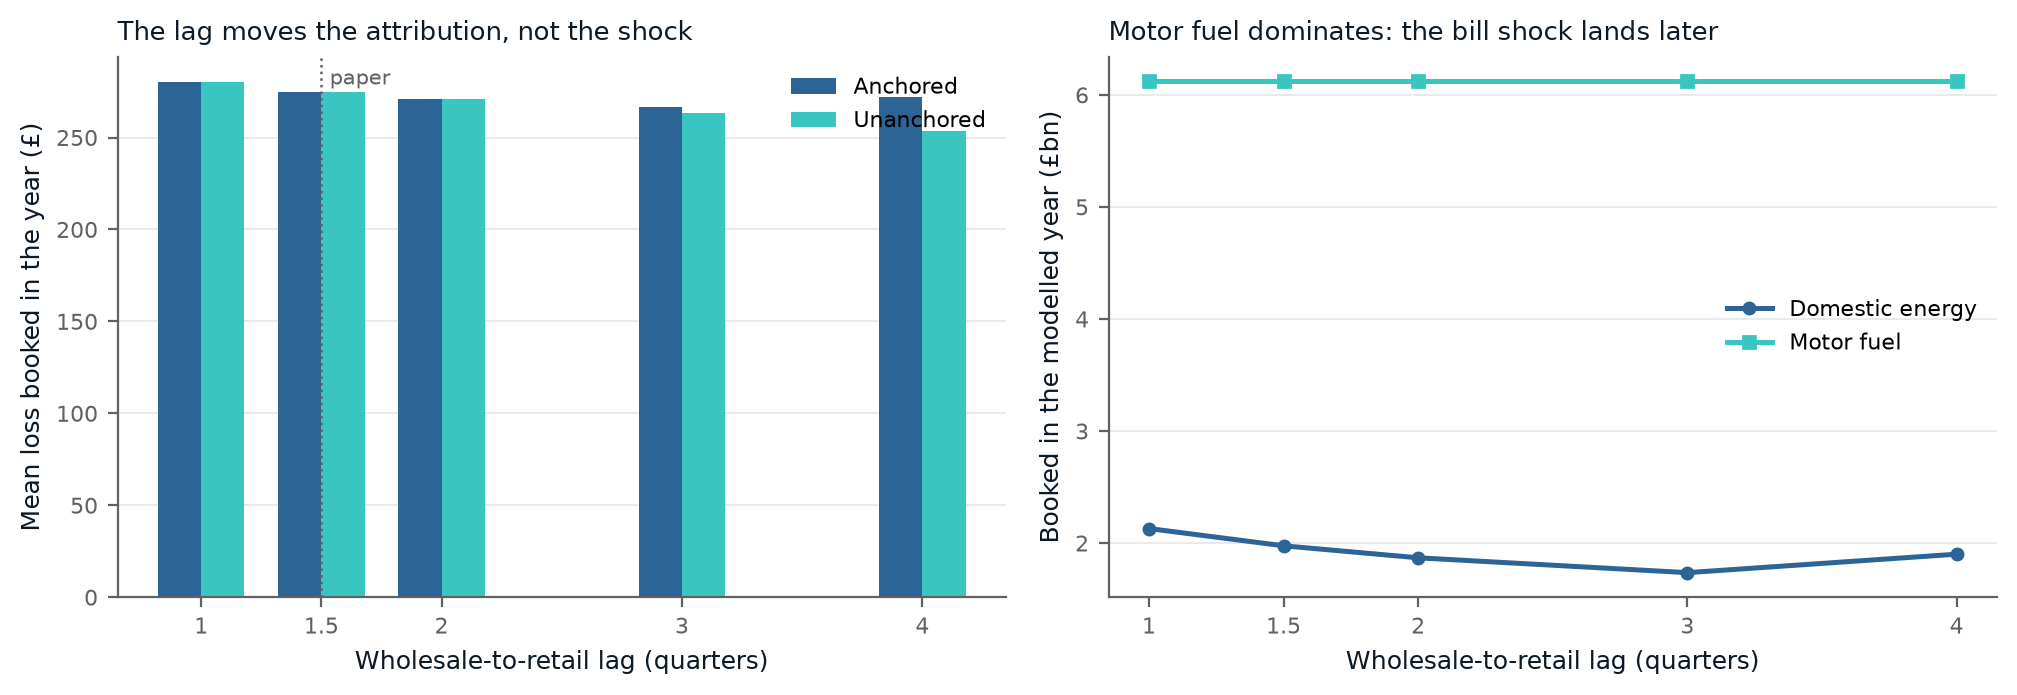
\includegraphics[width=.85\textwidth]{../results/figures/figA3_cap_lag.png}
\caption{Mean household loss over the modelled window under lags of one to four quarters, anchored and unanchored. The anchored series is the main specification's, with the gas sustained fraction re-solved at each lag against Ofgem's confirmed October cap; the unanchored series holds the fraction fixed. The gap between the two is how much of the lag sensitivity the anchor absorbs.}
\label{fig:caplag}
\end{figure}

\subsection{Marginal-pricing share: composition, not incidence}
\label{app:asymmetry}

The share of the time a gas-fired plant sets the GB marginal electricity price governs how far a wholesale gas move reaches the electricity cap. The main specification uses 0.85; setting it to 1.00 recovers the naive symmetric assumption that the move reaches electricity undamped, and 0.70 bounds it from below.

Stated plainly: it barely moves the answer. Going the whole way from 0.70 to 1.00 changes the mean household loss from \pounds\genAsymMeanLossLow{} to \pounds\genAsymMeanLossHigh{}, a difference of \genAsymMeanShiftPct{} per cent, and the decile-one to decile-ten percentage ratio is frozen at \genAsymRatioLow{} against \genAsymRatioHigh{} across the entire range. Nothing in the paper's distributional conclusions turns on this parameter, and Section~\ref{sec:step1} says so rather than claiming otherwise.

Where it does bite is composition, which is the one column that moves materially: the gas share of the domestic-energy loss falls from \genGasShareDomesticLow{} per cent at 0.70 to \genGasShareDomesticHigh{} per cent at 1.00, against \genGasShareDomesticCentral{} per cent in the main specification. Under the naive symmetric assumption the shock looks like an essentially even gas--electricity event; under the paper's calibration it is meaningfully gas-weighted. That matters for policy design and not for headline incidence: a gas-only social tariff, an electricity-side levy rebate, and the JRF block's choice of which unit rate to discount all land differently depending on which fuel carries the loss.

The honest summary is therefore narrow. The asymmetry is defensible on its merits and is the right modelling choice, but it is a compositional refinement rather than a load-bearing assumption. A reader who insists on the symmetric marginal-pricing assumption gets a mean loss \genAsymMeanShiftPct{} per cent larger and identical distributional conclusions. Note that this is the marginal-pricing share, not the gas-versus-pump damping ratio of Appendix~\ref{app:specvariants}: the first is a compositional refinement within the domestic leg, the second moves the motor-fuel share across the majority threshold. Confusing the two would understate how much of this paper's composition result is calibration.

% tab_asymmetry.tex — machine-generated by analysis/emit_tables.py
% generated 2026-08-26T13:05:57Z from results/ (central scenario: realised_2026). DO NOT EDIT BY HAND.
% A complete table float, caption and label included: the appendix inputs this directly. Requires \usepackage{booktabs}.
\begin{table}[htbp]
\centering
\caption{Marginal-pricing-share sweep, realised 2026 scenario. The gas price factor is held at 1.1404 throughout; only the electricity pass-through varies. The headline incidence barely moves, while the composition of the domestic loss moves materially.}
\label{tab:asymmetry}
{\small\setlength{\tabcolsep}{4.5pt}
\begin{tabular}{lrrrrrr}
\toprule
\begin{tabular}[b]{@{}l@{}}Marginal- \\ pricing share\end{tabular} & \begin{tabular}[b]{@{}c@{}}Electricity \\ factor\end{tabular} & \begin{tabular}[b]{@{}c@{}}Mean loss \\ (\pounds)\end{tabular} & \begin{tabular}[b]{@{}c@{}}Loss \\ (\% inc.)\end{tabular} & \begin{tabular}[b]{@{}c@{}}Decile \\ 1/10 ratio\end{tabular} & \begin{tabular}[b]{@{}c@{}}Gas share of \\ domestic loss (\%)\end{tabular} & \begin{tabular}[b]{@{}c@{}}Aggregate \\ (\pounds bn)\end{tabular} \\
\midrule
0.70 & 1.0764 & 331 & 0.54 & 5.68 & 59.3 & 9.76 \\
0.85 (paper) & 1.0928 & 343 & 0.56 & 5.68 & 54.6 & 10.12 \\
1.00 & 1.1092 & 356 & 0.58 & 5.67 & 50.5 & 10.48 \\
\bottomrule
\end{tabular}
}
\end{table}


\subsection{The scenario grid: when does the shock stop being a pump-price event?}
\label{app:grid}

The three named scenarios are points, and a reader is entitled to ask how much of the paper's argument is an artefact of where those points happen to sit. Figure~\ref{fig:grid} answers that by sweeping the two drivers against each other: a wholesale gas move, which reaches households through the regulated cap, against a crude oil move, which reaches them at the pump. Every cell is built through the same pass-through machinery as the named scenarios and scored on the same baseline, so the grid is a genuine extension of the main specification rather than a separate exercise.

\begin{figure}[htbp]
\centering
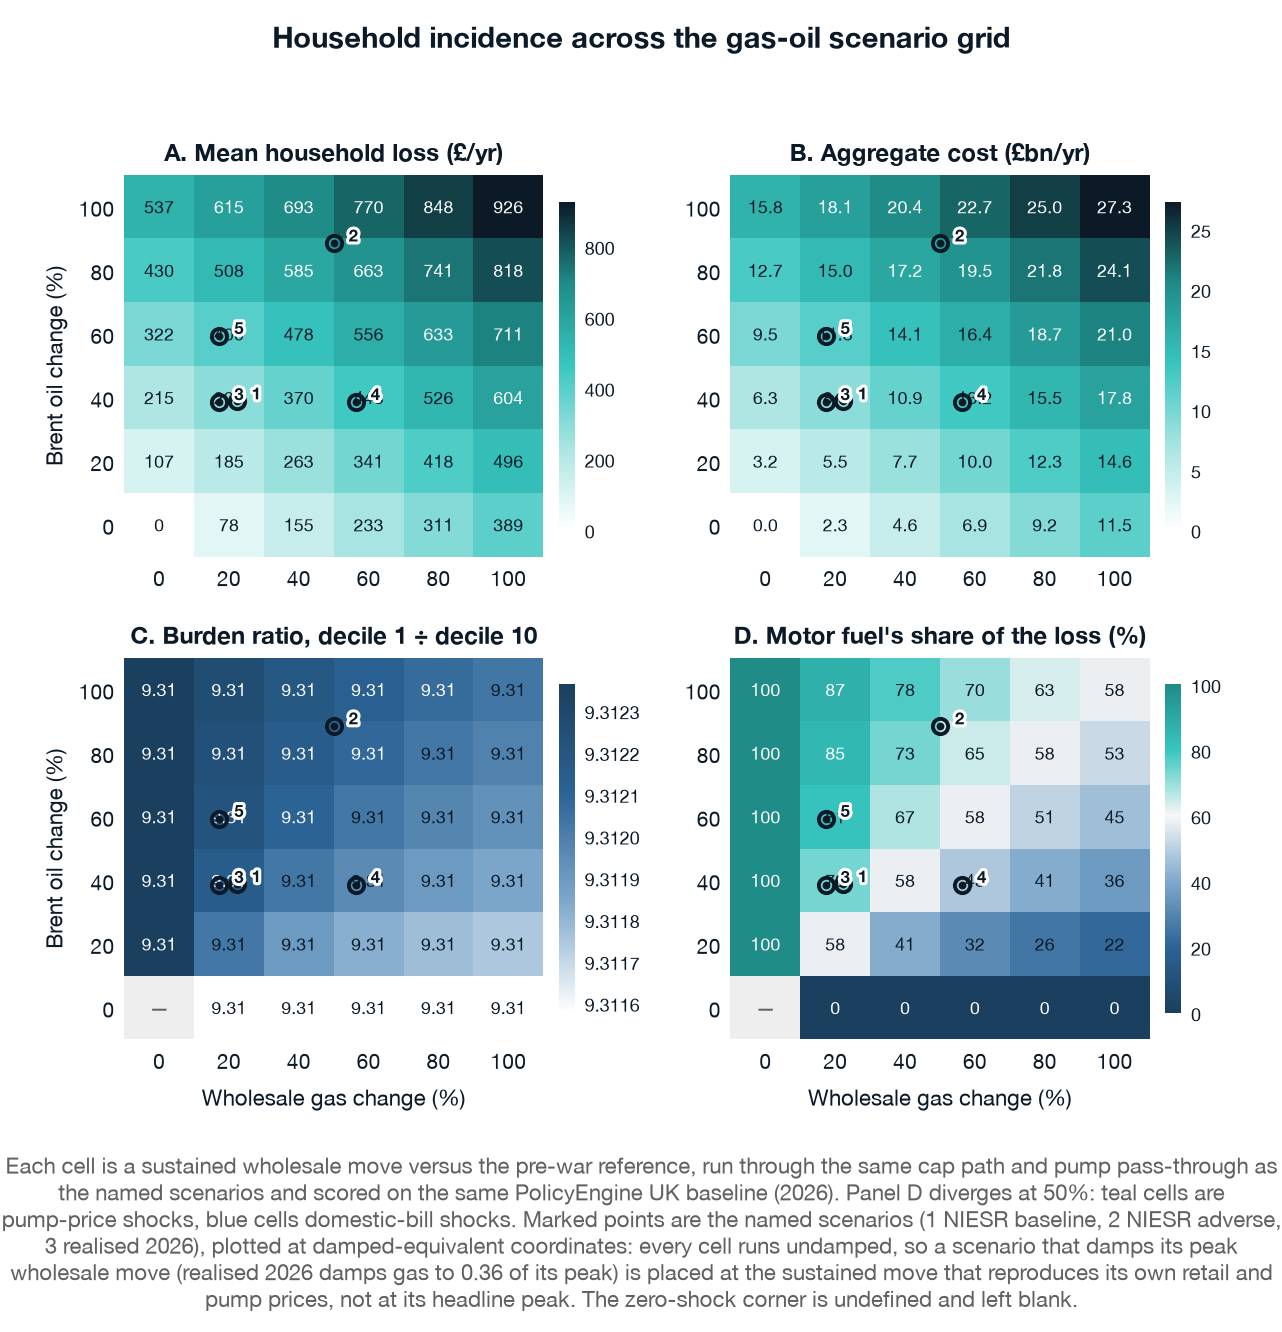
\includegraphics[width=\textwidth]{../results/figures/fig_scenario_grid.png}
\caption{Household incidence across the gas--oil scenario grid. Panel D diverges at fifty per cent: shaded one way the shock is a pump-price event, the other a domestic-bill event. Marked points are the three named scenarios.}
\label{fig:grid}
\end{figure}

One correction has to come before the results, because an earlier version of this appendix reported grid decile ratios that no reader could reconcile with the rest of the paper. The published grid gave decile-one to decile-ten burden ratios of 11.77 to 12.73, outside the range of every specification in the paper, with no reconciliation offered. Those figures were a stale artefact: they were computed on the unequivalised denominator this revision replaces (Section~\ref{sec:step2}), while the named scenarios had already moved to the equivalised one. Regenerated on the paper's own denominator, every cell of the grid returns \genDomesticOnlyDecileRatioPct{} to one, consistent with the domestic-only ratio the named scenarios produce. The consistency is now enforced rather than asserted: the burden ratio is an aggregate ratio and therefore scale-invariant, so a named scenario differs from a grid cell only in its channel mix and any mix must produce a ratio bracketed by the two pure-channel cells. \texttt{run\_grid.py} checks every named scenario against the live grid's range and \emph{raises} if one falls outside it, so a grid and a headline produced by different code cannot both be published again.

Two things follow. The first is that the distributional gradient is invariant to the mix. The decile-one to decile-ten burden ratio moves only between \genGridRatioMin{} and \genGridRatioMax{} across the entire grid, so the paper's central finding --- that the burden falls steeply in income even where the cash loss does not --- does not depend on which driver carries the shock. That near-degeneracy is itself informative rather than reassuring: the domestic and motor-fuel channels turn out to have almost the same decile gradient in this imputation, which is the fuel-imputation defect of Section~\ref{sec:limitations} --- deciles one and ten recording the same fuel-purchasing rate --- showing up from a different direction. The gradient is a property of how the imputed energy and fuel budget shares vary with income, and the flatness of the grid is a reminder that one of those two profiles is known to be wrong.

The second is a boundary. Motor fuel ceases to carry the larger share of the loss along a frontier at roughly \genGridFrontierSlope{} times as large a proportional gas move as oil move; below that line the shock is predominantly a pump-price event and above it predominantly a domestic-bill one. One caution about reading the named scenarios against that frontier: every cell of the grid is run undamped, and the named scenarios are plotted at their undamped coordinates, so the comparison is not like-for-like with the damped main specification whose motor-fuel share Section~\ref{sec:results-fuel} reports. An earlier version of this appendix asserted that all three named scenarios sit below the frontier; on the grid's own undamped numbers that is not established, and the claim is withdrawn. What the grid does show is that the frontier exists, that it is not far from the region a gas-and-oil shock of this kind occupies, and that which side of it a given shock falls on depends on the damping calibration --- which is the same calibration dependence Section~\ref{sec:results-fuel} reports, arriving here from a different direction.


\subsection{The common exchequer envelope, and its four row types}
\label{app:envelope}

Table~\ref{tab:envelope} reports every instrument at each of the four row types set out in Section~\ref{sec:step4}: at the sponsor's own stated cost, at the instrument's feasible maximum, at a parameter scaled past that maximum until the \pounds \genEnvelopeBn{} billion envelope is exhausted, and at widened eligibility with generosity held at the sponsor's own parameter. Each row carries a feasibility flag and, where the instrument cannot absorb the envelope, the amount it can absorb.

The table is the arithmetic behind the withdrawal in Section~\ref{sec:policy}. VAT zero-rating absorbs \pounds \genVatCutCostBn{} billion --- the whole of the five-point reduced rate --- so its feasible-maximum row and its stated-cost row coincide and no scaling makes it a \pounds \genEnvelopeBn{} billion instrument; the social tariff absorbs \pounds \genSocialTariffAbsorbableBn{} billion and the Warm Home Discount expansion \pounds \genWhdAbsorbableBn{} billion. The three scaled rows that exceed a feasible maximum are labelled generically --- a proportional domestic-bill subsidy at \genSocialTariffScaledParameterPct{} per cent on the means-tested population, a flat payment of \pounds \genWhdScaledParameterGbp{} a year to the same population, and a proportional domestic-bill subsidy at \genVatCutScaledParameterPct{} per cent universally --- because none of them is the policy whose name it used to carry. The eligibility rows are feasible throughout, and the comparison between them and the feasible-maximum rows is the finding of Section~\ref{sec:policy-eligibility}.

\begin{figure}[htbp]
\centering
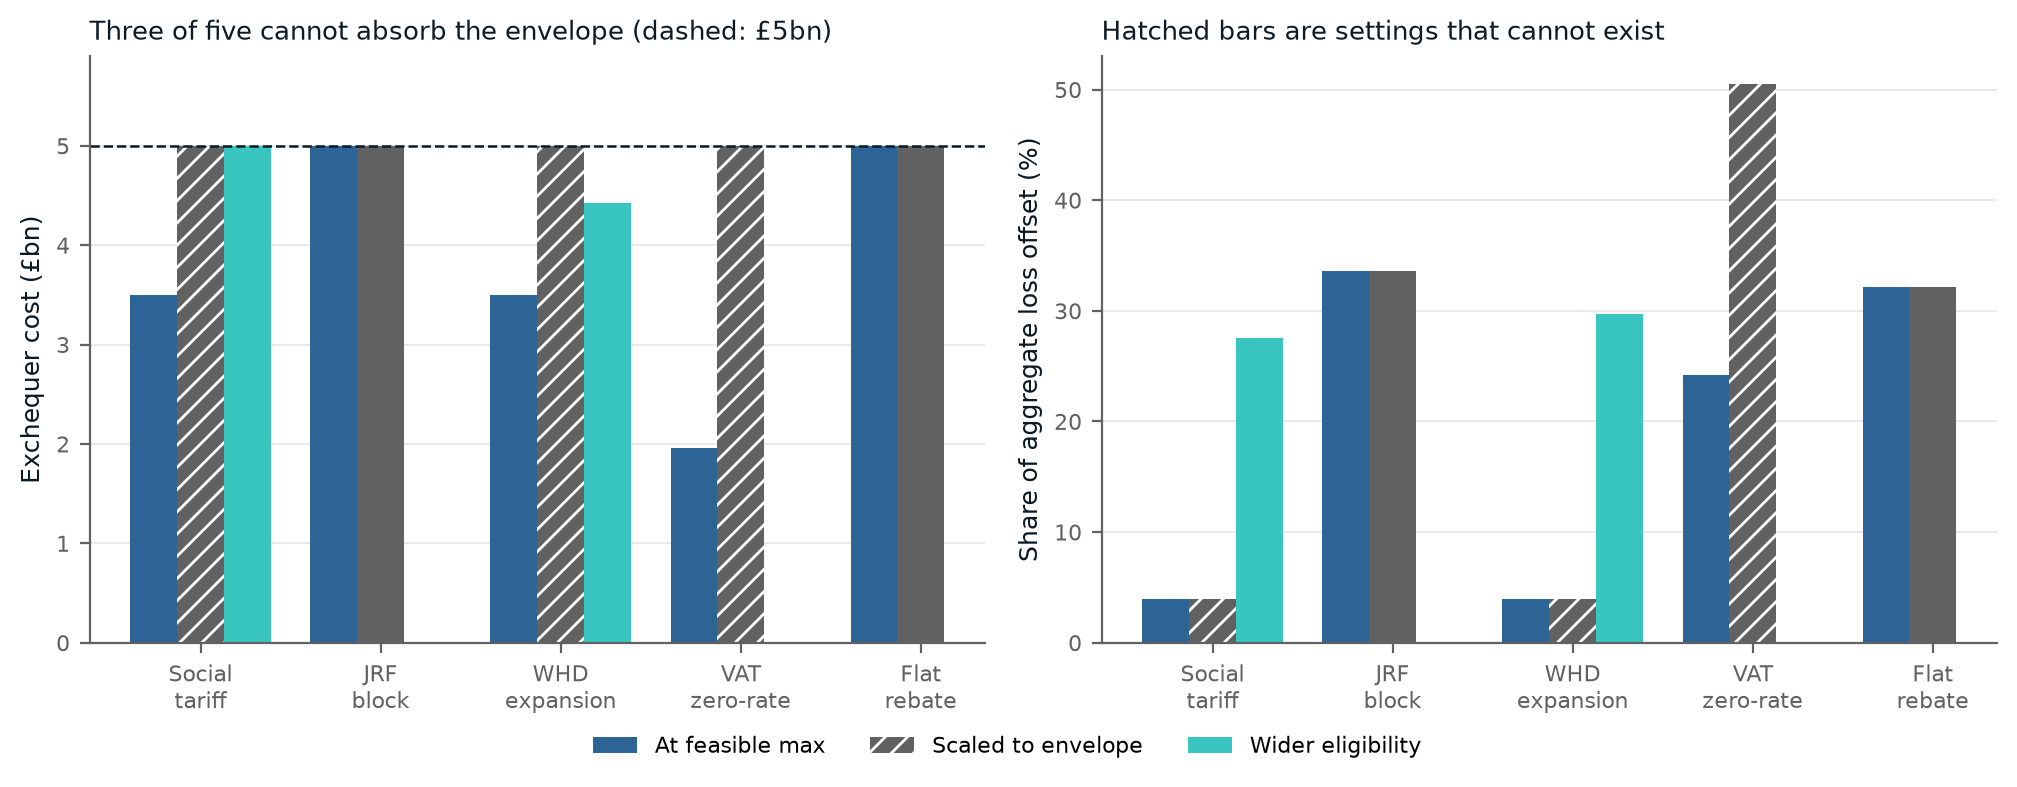
\includegraphics[width=\textwidth]{../results/figures/figA4_policy_envelope.png}
\caption{The five instruments at a common exchequer envelope. Rows whose implied parameter does not exist are marked: the ranking they generate is not a ranking of the policies named. Widening eligibility at each sponsor's own generosity offsets far more of the loss than deepening the discount at fixed eligibility.}
\label{fig:envelope}
\end{figure}

% tab_envelope.tex — machine-generated by analysis/emit_tables.py
% generated 2026-08-27T11:36:28Z from results/ (central scenario: realised_2026). DO NOT EDIT BY HAND.
% A complete table float, caption and label included: the appendix inputs this directly. Requires \usepackage{booktabs}.
\begin{table}[htbp]
\centering
\caption{The five instruments against a common exchequer envelope of \pounds 5bn, realised 2026 scenario. The first two rows for each instrument answer different questions and the pre-revision table conflated them. ``Own ceiling'' is the instrument at its own feasible maximum with no envelope applied at all: the JRF block reaches \pounds 21.9bn there, more than 4 times the envelope. ``Absorbs envelope'' is the budget constraint --- the smaller of the envelope and that ceiling --- so for an instrument that already costs more than \pounds 5bn it scales generosity \emph{down}, and for the three that saturate below the envelope it reports the smaller sum they can actually spend. Neither row holds spend fixed across instruments. ``Scaled'' is proportional scaling to the full envelope regardless of feasibility; $\dagger$ marks the three rows whose implied setting does not exist (a bill discount above 100 per cent, more VAT points than the tax has). ``Wider eligibility'' spends the envelope on who is in the scheme rather than on how generous it is, at the sponsor's own rate, and is defined only for the two means-tested schemes; $\ddagger$ marks the four such rows where widening reaches every household, at which point the instrument is means-tested in name only. Any claim that one instrument ``wins at a common envelope'' rests on the scaled rows and is withdrawn.}
\label{tab:envelope}
{\small\setlength{\tabcolsep}{2.6pt}
\begin{tabular}{llrrrrrr}
\toprule
Instrument & Variant & \begin{tabular}[b]{@{}c@{}}Spend \\ (\pounds bn)\end{tabular} & \begin{tabular}[b]{@{}c@{}}Implied \\ setting\end{tabular} & \begin{tabular}[b]{@{}c@{}}Share to \\ D1--3 (\%)\end{tabular} & \begin{tabular}[b]{@{}c@{}}Loss \\ offset (\%)\end{tabular} & \begin{tabular}[b]{@{}c@{}}Mean res- \\ idual (\pounds)\end{tabular} & \begin{tabular}[b]{@{}c@{}}Un-comp- \\ ensated (\%)\end{tabular} \\
\midrule
Social tariff & own ceiling & 3.76 & 100\% & 57.5 & 5.2 & 357 & 84 \\
 & absorbs envelope & 3.76 & 100\% & 57.5 & 5.2 & 357 & 84 \\
 & scaled & 5.00 & 133\%$^\dagger$ & 57.5 & 5.2 & 357 & 84 \\
 & wider eligibility & 5.00 & 35\% & 71.7 & 26.6 & 276 & 62 \\
\addlinespace
JRF block & own ceiling & 21.86 & 100\% & 29.7 & 70.5 & 111 & 10 \\
 & absorbs envelope & 5.00 & 22.9\% & 29.7 & 36.1 & 241 & 41 \\
 & scaled & 5.00 & 22.9\% & 29.7 & 36.1 & 241 & 41 \\
\addlinespace
WHD expansion & own ceiling & 3.76 & \pounds 814 & 60.0 & 5.1 & 357 & 85 \\
 & absorbs envelope & 3.76 & \pounds 814 & 60.0 & 5.1 & 357 & 85 \\
 & scaled & 5.00 & \pounds 1,083$^\dagger$ & 60.0 & 5.2 & 357 & 84 \\
 & wider eligibility$^\ddagger$ & 4.42 & \pounds 150 & 30.0 & 29.3 & 266 & 49 \\
\addlinespace
VAT zero-rate & own ceiling & 2.11 & 5\% & 24.7 & 19.0 & 305 & 100 \\
 & absorbs envelope & 2.11 & 5\% & 24.7 & 19.0 & 305 & 100 \\
 & scaled & 5.00 & 11.9\%$^\dagger$ & 24.7 & 44.9 & 208 & 78 \\
\addlinespace
Flat rebate & own ceiling$^\ddagger$ & 5.39 & \pounds 183 & 30.0 & 33.2 & 251 & 43 \\
 & absorbs envelope$^\ddagger$ & 5.00 & \pounds 170 & 30.0 & 31.7 & 257 & 45 \\
 & scaled$^\ddagger$ & 5.00 & \pounds 170 & 30.0 & 31.7 & 257 & 45 \\
\bottomrule
\end{tabular}
}
\end{table}


\subsection{The domestic leg: what the anchor does and does not pin}
\label{app:domesticleg}

Table~\ref{tab:domesticleg} sweeps the parameters that scale the domestic channel one for one and are not otherwise identified. The gas sustained fraction and the phase-in weight at the anchor quarter enter the cap only as a product, so the confirmed-cap anchor pins the product and not the split; the sweep varies the split at a fixed product to show that the headline is insensitive to it. It also varies the three parameters the anchor does not touch --- the pre-war NBP gas price, and the wholesale shares of the gas and electricity bills --- which move the domestic leg proportionally and therefore move the motor-fuel share, between \genDomesticLegNbpFuelShareMinPct{} and \genDomesticLegNbpFuelShareMaxPct{} per cent on the pre-war gas price alone. That is the largest single-parameter movement in the composition result and it is why Section~\ref{sec:results-fuel} quotes a range.

% tab_domestic_leg.tex — machine-generated by analysis/emit_tables.py
% generated 2026-08-26T15:20:08Z from results/ (central scenario: realised_2026). DO NOT EDIT BY HAND.
% A complete table float, caption and label included: the appendix inputs this directly. Requires \usepackage{booktabs}.
\begin{table}[htbp]
\centering
\caption{Domestic-leg parameter sweep, realised 2026 scenario. The Cornwall Insight anchor identifies only the product of the sustained fraction and the first phase-in quarter, so the first block varies the split at a constant product; the remaining blocks vary the three parameters that scale the domestic channel one for one. The aggregate, and with it the motor-fuel share, is materially sensitive to this calibration.}
\label{tab:domesticleg}
{\small\setlength{\tabcolsep}{2.6pt}
\begin{tabular}{llrrrrrr}
\toprule
Parameter & \begin{tabular}[b]{@{}l@{}}Value\end{tabular} & \begin{tabular}[b]{@{}c@{}}Agg. \\ (\pounds bn)\end{tabular} & \begin{tabular}[b]{@{}c@{}}Mean \\ (\pounds)\end{tabular} & \begin{tabular}[b]{@{}c@{}}Mean \\ (\%)\end{tabular} & \begin{tabular}[b]{@{}c@{}}D1 \\ (\%)\end{tabular} & \begin{tabular}[b]{@{}c@{}}D10 \\ (\%)\end{tabular} & \begin{tabular}[b]{@{}c@{}}Motor fuel \\ (\% of loss)\end{tabular} \\
\midrule
Sustained fraction & 0.18 & 7.54 & 256 & 0.56 & 2.13 & 0.23 & 74.9 \\
 & 0.24 & 8.01 & 272 & 0.60 & 2.27 & 0.25 & 70.5 \\
 & 0.3 & 8.49 & 288 & 0.63 & 2.41 & 0.26 & 66.6 \\
 & 0.36 (paper) & 8.96 & 304 & 0.67 & 2.55 & 0.28 & 63.1 \\
 & 0.45 & 9.67 & 328 & 0.72 & 2.75 & 0.30 & 58.5 \\
 & 0.6 & 10.85 & 368 & 0.81 & 3.09 & 0.33 & 52.1 \\
 & 0.72 & 11.79 & 400 & 0.88 & 3.37 & 0.36 & 47.9 \\
\midrule
Pre-war NBP & 70 & 9.90 & 336 & 0.74 & 2.82 & 0.31 & 57.1 \\
 & 80 & 9.37 & 318 & 0.70 & 2.67 & 0.29 & 60.3 \\
 & 90 (paper) & 8.96 & 304 & 0.67 & 2.55 & 0.28 & 63.1 \\
 & 100 & 8.63 & 293 & 0.64 & 2.45 & 0.27 & 65.5 \\
 & 110 & 8.36 & 284 & 0.62 & 2.37 & 0.26 & 67.6 \\
 & 130 & 7.94 & 269 & 0.59 & 2.25 & 0.24 & 71.2 \\
\midrule
Wholesale share, gas & 0.35 & 8.56 & 291 & 0.64 & 2.43 & 0.26 & 66.0 \\
 & 0.4 & 8.76 & 297 & 0.65 & 2.49 & 0.27 & 64.5 \\
 & 0.45 (paper) & 8.96 & 304 & 0.67 & 2.55 & 0.28 & 63.1 \\
 & 0.5 & 9.15 & 311 & 0.68 & 2.60 & 0.28 & 61.7 \\
 & 0.55 & 9.35 & 317 & 0.70 & 2.66 & 0.29 & 60.4 \\
\midrule
Wholesale share, elec. & 0.25 & 8.52 & 289 & 0.63 & 2.42 & 0.26 & 66.3 \\
 & 0.3 & 8.74 & 297 & 0.65 & 2.48 & 0.27 & 64.7 \\
 & 0.35 (paper) & 8.96 & 304 & 0.67 & 2.55 & 0.28 & 63.1 \\
 & 0.4 & 9.18 & 311 & 0.68 & 2.61 & 0.28 & 61.6 \\
 & 0.45 & 9.39 & 319 & 0.70 & 2.67 & 0.29 & 60.1 \\
\bottomrule
\end{tabular}
}
\end{table}


\subsection{Upstream contributions arising}
\label{app:upstream}

Three of this paper's limitations are model gaps rather than data gaps, and each is precise enough to fix. They are contributed upstream to PolicyEngine UK rather than only reported here: a live price channel for the imputed energy variables, so that a cap or pump-price reform moves household spend rather than silently cutting quantities; a Warm Home Discount parameter and variable, which the model currently lacks entirely; and a primary-heating-fuel or gas-grid indicator in the microdata, without which the off-gas-grid question in Section~\ref{sec:discussion} cannot be asked of any UK microsimulation.

Three calibration findings from this paper's validation work are contributed alongside them, because both are properties of the model rather than of this application. The first is the motor-fuel imputation: the imputed decile profile of motor-fuel spend is almost flat, \pounds \genFuelSpendDecileOneRawGbp{} against \pounds \genFuelSpendDecileTenRawGbp{}, where the ONS Family Spending profile runs \pounds \genOnsBenchFuelDecileOneGbp{} to \pounds \genOnsBenchFuelDecileTenGbp{} \citep{ons2026familyspending}, both annualised at $365.25/7 = 52.18$ weeks rather than at 52, and the fuel-purchasing participation rate is identical in deciles one and ten where the Department for Transport's National Travel Survey table on household car \emph{availability} shows 40 per cent of the poorest quintile without a car against 14 per cent of the richest \citep{dft2025nts} --- a table covering England only, while the model is UK-wide, so it bounds the direction of the defect rather than measuring it. The second is domestic energy, imputed in the opposite direction: mean modelled domestic spend of \pounds \genModelDomesticMeanGbp{} against ONS Family Spending's \pounds \genOnsBenchDomesticMeanGbp{} \citep{ons2026familyspending} and DESNZ's fixed-consumption dual-fuel bill \citep{desnz2026qep}, roughly a quarter low, and below the typical-consumption cap level, which a population mean should not be. The two run opposite ways and compound on the fuel share, so they are reported together. The third is means-tested coverage: the model's entire means-tested population, \genMeansTestedHouseholdsM{} million households, sits well below the 7.2 million households on Universal Credit alone in May 2026. All three are quantified against published administrative and survey benchmarks and are reported upstream in that form. The contributed energy-bills parameter that no variable reads is separately flagged for removal or implementation.

\subsection{Reproduction}
\label{app:reproduce}

This subsection is the one place in the paper where implementation detail is given, because reproduction requires it.

All code, parameters and aggregate results are in the paper's public repository; the microdata are not. PolicyEngine UK's enhanced Family Resources Survey dataset is held in a private repository under a licence that does not permit redistribution, so reproducing the household-level results requires an access token. The aggregate outputs are committed, so every number in the paper can be traced from the stored artefacts to the macro that renders it without re-running the microsimulation:

\begin{itemize}\setlength{\itemsep}{0pt}
  \item \texttt{analysis/run\_incidence.py} --- baseline, shock and policy scoring
  \item \texttt{analysis/run\_variants.py} --- the specification variants of Appendix~\ref{app:specvariants}
  \item \texttt{analysis/run\_sensitivity.py} --- the elasticity, cap-lag and marginal-pricing sweeps
  \item \texttt{analysis/run\_grid.py} --- the scenario grid of Figure~\ref{fig:grid}
  \item \texttt{analysis/emit\_tex\_values.py} --- every numeric macro used in the text
\end{itemize}
The model gaps recorded in Section~\ref{sec:limitations} correspond to open issues in the \texttt{policyengine-uk} repository: the absence of a demand-elasticity and pass-through block is issue \#1114, and the unvalidated 0.38 VAT coverage factor is issue \#352.

\begin{verbatim}
uv sync
export HUGGING_FACE_TOKEN=hf_...     # needs private dataset access
python analysis/run_incidence.py     # scenarios + policies -> results/*.json
python analysis/run_variants.py      # the seven specifications
python analysis/run_sensitivity.py   # the four sweeps
python analysis/run_grid.py          # scenario grid -> results/grid/*.csv
python analysis/emit_tables.py       # results/ -> paper/tables/*.tex
python analysis/emit_tex_values.py   # -> paper/values_generated.tex
python -m pytest tests/              # runs without microdata
cd paper && latexmk -pdf main.tex
\end{verbatim}

Every headline number enters the prose as a macro from \texttt{paper/values\_generated.tex}, emitted mechanically from \texttt{results/}. A macro with no corresponding key in \texttt{results/} renders as \texttt{\textbackslash GENMISSING}, so a stale or partial results tree fails visibly in the compiled document rather than silently preserving superseded numbers. This is also why no constituency-level or heating-fuel statistic appears anywhere in the paper: with no key in \texttt{results/} to back it, no such number can be rendered. Pinned dependency versions, including the \texttt{policyengine-uk} release used, are in \texttt{pyproject.toml} and \texttt{uv.lock}.
